% vim: set spell spelllang=en tw=100 et sw=4 sts=4 foldmethod=marker foldmarker={{{,}}} :

\documentclass{beamer}

\usepackage{tikz}
\usepackage{xcolor}
\usepackage{complexity}
\usepackage{hyperref}
\usepackage{microtype}
\usepackage{amsmath}                   % \operatorname
\usepackage{amsfonts}                  % \mathcal
\usepackage{amssymb}                   % \nexists
\usepackage[vlined]{algorithm2e} % algorithms
\usepackage{centernot}
\usepackage{fancyvrb}

\RequirePackage[tt=false, type1=true]{libertine}
\RequirePackage[varqu]{zi4}
\RequirePackage[libertine]{newtxmath}
\RequirePackage[T1]{fontenc}

\usepackage{bussproofs}
\usepackage{stmaryrd}

\usepackage[formats]{listings}
\lstset{
    morecomment=[f]*,
    basicstyle=\ttfamily,
    commentstyle=\color{uofgcobalt}
}

\newcommand*{\rom}[1]{\emph{\romannumeral #1 \relax}}
\newcommand{\neighbourhood}{\operatorname{N}}
\newcommand{\vertexset}{\operatorname{V}}

\usetikzlibrary{shapes, arrows, shadows, calc, positioning, fit}
\usetikzlibrary{decorations.pathreplacing, decorations.pathmorphing, shapes.misc}
\usetikzlibrary{tikzmark}
\usetikzlibrary{trees}
\usetikzlibrary{backgrounds}

\definecolor{uofguniversityblue}{rgb}{0, 0.219608, 0.396078}

\definecolor{uofgheather}{rgb}{0.356863, 0.32549, 0.490196}
\definecolor{uofgaquamarine}{rgb}{0.603922, 0.72549, 0.678431}
\definecolor{uofgslate}{rgb}{0.309804, 0.34902, 0.380392}
\definecolor{uofgrose}{rgb}{0.823529, 0.470588, 0.709804}
\definecolor{uofgmocha}{rgb}{0.709804, 0.564706, 0.47451}
\definecolor{uofgsandstone}{rgb}{0.321569, 0.278431, 0.231373}
\definecolor{uofgforest}{rgb}{0, 0.2, 0.129412}
\definecolor{uofglawn}{rgb}{0.517647, 0.741176, 0}
\definecolor{uofgcobalt}{rgb}{0, 0.615686, 0.92549}
\definecolor{uofgturquoise}{rgb}{0, 0.709804, 0.819608}
\definecolor{uofgsunshine}{rgb}{1.0, 0.862745, 0.211765}
\definecolor{uofgpumpkin}{rgb}{1.0, 0.72549, 0.282353}
\definecolor{uofgthistle}{rgb}{0.584314, 0.070588, 0.447059}
\definecolor{uofgrust}{rgb}{0.603922, 0.227451, 0.023529}
\definecolor{uofgburgundy}{rgb}{0.490196, 0.133333, 0.223529}
\definecolor{uofgpillarbox}{rgb}{0.701961, 0.047059, 0}
\definecolor{uofglavendar}{rgb}{0.356863, 0.301961, 0.580392}

\tikzset{vertex/.style={draw, circle, inner sep=0pt, minimum size=0.5cm, font=\small\bfseries}}
\tikzset{notvertex/.style={vertex, color=white, text=black}}
\tikzset{plainvertex/.style={vertex}}
\tikzset{vertexc1/.style={vertex, fill=uofgburgundy, text=white}}
\tikzset{vertexc2/.style={vertex, fill=uofgsandstone, text=white}}
\tikzset{vertexc3/.style={vertex, fill=uofgforest, text=white}}
\tikzset{vertexc4/.style={vertex, fill=uofgheather, text=white}}
\tikzset{edge/.style={color=black!50!white}}
\tikzset{bedge/.style={ultra thick}}

% {{{ theme things
\useoutertheme[footline=authortitle]{miniframes}
\useinnertheme{rectangles}

\setbeamerfont{block title}{size={}}
\setbeamerfont{title}{size=\large,series=\bfseries}
\setbeamerfont{section title}{size=\large,series=\mdseries}
\setbeamerfont{author}{size=\normalsize,series=\mdseries}
\setbeamercolor*{structure}{fg=uofguniversityblue}
\setbeamercolor*{palette primary}{use=structure,fg=black,bg=white}
\setbeamercolor*{palette secondary}{use=structure,fg=white,bg=uofgcobalt}
\setbeamercolor*{palette tertiary}{use=structure,fg=white,bg=uofguniversityblue}
\setbeamercolor*{palette quaternary}{fg=white,bg=black}

\setbeamercolor*{titlelike}{parent=palette primary}

\beamertemplatenavigationsymbolsempty

\setbeamertemplate{title page}
{
    \begin{tikzpicture}[remember picture, overlay]
        \node at (current page.north west) {
            \begin{tikzpicture}[remember picture, overlay]
                \fill [fill=uofguniversityblue, anchor=north west] (0, 0) rectangle (\paperwidth, -3.0cm);
            \end{tikzpicture}
        };

        \node (logo) [anchor=north east, shift={(-0.2cm,-0.1cm)}] at (current page.north east) {
            \includegraphics[keepaspectratio=true,scale=0.5]{UoG_keyline.pdf}
        };

        \node (morelogo) [anchor=north, below=0.15cm of logo.south] {
            \raisebox{0.05cm}{\includegraphics[keepaspectratio=true,scale=0.045]{ucph.png}}\hspace*{0.5cm}
            \includegraphics[keepaspectratio=true,scale=0.08]{LundUniversity_C2line_NEG.png}
        };

        \node [anchor=west, xshift=0.2cm, yshift=-0.8cm] at (current page.west |- logo.west) {
            \begin{minipage}{0.7\paperwidth}\raggedright
                {\usebeamerfont{title}\usebeamercolor[white]{}\inserttitle}\\[0.1cm]
                {\usebeamerfont{author}\usebeamercolor[white]{}\insertauthor}
            \end{minipage}
        };
    \end{tikzpicture}
}

\setbeamertemplate{section page}
{
    \begin{centering}
        \begin{beamercolorbox}[sep=12pt,center]{part title}
            \usebeamerfont{section title}\insertsection\par
        \end{beamercolorbox}
    \end{centering}
}

\newcommand{\frameofframes}{/}
\newcommand{\setframeofframes}[1]{\renewcommand{\frameofframes}{#1}}

\makeatletter
\setbeamertemplate{footline}
{%
    \begin{beamercolorbox}[colsep=1.5pt]{upper separation line foot}
    \end{beamercolorbox}
    \begin{beamercolorbox}[ht=2.5ex,dp=1.125ex,%
        leftskip=.3cm,rightskip=.3cm plus1fil]{author in head/foot}%
        \leavevmode{\usebeamerfont{author in head/foot}\insertshortauthor}%
        \hfill%
        {\usebeamerfont{institute in head/foot}\usebeamercolor[fg]{institute in head/foot}\insertshortinstitute}%
    \end{beamercolorbox}%
    \begin{beamercolorbox}[ht=2.5ex,dp=1.125ex,%
        leftskip=.3cm,rightskip=.3cm plus1fil]{title in head/foot}%
        {\usebeamerfont{title in head/foot}\insertshorttitle}%
        \hfill%
        {\usebeamerfont{frame number}\usebeamercolor[fg]{frame number}\insertframenumber~\frameofframes~\inserttotalframenumber}
    \end{beamercolorbox}%
    \begin{beamercolorbox}[colsep=1.5pt]{lower separation line foot}
    \end{beamercolorbox}
}

\makeatletter
\newenvironment{nearlyplainframe}[2][]{
    \def\beamer@entrycode{\vspace*{-\headheight}\vspace*{3pt}}
    \setbeamertemplate{headline}
    {%
        \begin{beamercolorbox}[colsep=1.5pt]{upper separation line head}
        \end{beamercolorbox}
        \begin{beamercolorbox}[ht=0.5ex,dp=0.125ex,%
            leftskip=.3cm,rightskip=.3cm plus1fil]{title in head/foot}%
        \end{beamercolorbox}%
        \begin{beamercolorbox}[ht=0.5ex,dp=0.125ex,%
            leftskip=.3cm,rightskip=.3cm plus1fil]{author in head/foot}%
        \end{beamercolorbox}%
        \begin{beamercolorbox}[colsep=1.5pt]{lower separation line head}
        \end{beamercolorbox}
        \vspace*{\headheight}
    }

    \setbeamertemplate{footline}
    {%
        \begin{beamercolorbox}[colsep=1.5pt]{upper separation line foot}
        \end{beamercolorbox}
        \begin{beamercolorbox}[ht=0.5ex,dp=0.125ex,%
            leftskip=.3cm,rightskip=.3cm plus1fil]{author in head/foot}%
        \end{beamercolorbox}%
        \begin{beamercolorbox}[ht=0.5ex,dp=0.125ex,%
            leftskip=.3cm,rightskip=.3cm plus1fil]{title in head/foot}%
        \end{beamercolorbox}%
        \begin{beamercolorbox}[colsep=1.5pt]{lower separation line foot}
        \end{beamercolorbox}
    }

    \begin{frame}[#1]{#2}
    }{
    \end{frame}
}
\makeatother

\makeatletter
\newenvironment{justborderframe}[2][]{
    \def\beamer@entrycode{\vspace*{-\headheight}}
    \setbeamertemplate{headline}
    {%
        \begin{beamercolorbox}[colsep=1.5pt]{upper separation line head}
        \end{beamercolorbox}
        \begin{beamercolorbox}[ht=0.5ex,dp=0.125ex,%
            leftskip=.3cm,rightskip=.3cm plus1fil]{title in head/foot}%
        \end{beamercolorbox}%
        \begin{beamercolorbox}[ht=0.5ex,dp=0.125ex,%
            leftskip=.3cm,rightskip=.3cm plus1fil]{author in head/foot}%
        \end{beamercolorbox}%
        \begin{beamercolorbox}[colsep=1.5pt]{lower separation line head}
        \end{beamercolorbox}
        \vspace*{\headheight}
    }

    \setbeamertemplate{footline}
    {%
        \begin{beamercolorbox}[colsep=1.5pt]{upper separation line foot}
        \end{beamercolorbox}
        \begin{beamercolorbox}[ht=0.5ex,dp=0.125ex,%
            leftskip=.3cm,rightskip=.3cm plus1fil]{author in head/foot}%
        \end{beamercolorbox}%
        \begin{beamercolorbox}[ht=0.5ex,dp=0.125ex,%
            leftskip=.3cm,rightskip=.3cm plus1fil]{title in head/foot}%
        \end{beamercolorbox}%
        \begin{beamercolorbox}[colsep=1.5pt]{lower separation line foot}
        \end{beamercolorbox}
    }

    \begin{frame}[#1]{}
    }{
    \end{frame}
}
\makeatother


% }}}

\author{
    Stephan Gocht
    \and Ciaran McCreesh
    \and Jakob Nordstr\"{o}m}

\title{VeriPB: The Easy Way to Make Your Combinatorial Search Algorithm Trustworthy}

\begin{document}

{
    \usebackgroundtemplate{
        \tikz[overlay, remember picture]
        \node[at=(current page.south), anchor=south, inner sep=0pt]{\includegraphics[keepaspectratio=true, height=\paperheight]{background.jpg}};
    }
    \begin{frame}[plain,noframenumbering]
        \titlepage
    \end{frame}
}

\begin{frame}{The Problem}
    \begin{itemize}
        \item There are a lot of dedicated solvers for hard problems.
        \item Several of them are buggy\ldots
            \begin{itemize}
                \item \ldots including ones often regarded as ``state of the art''.
                \item But even the buggy ones nearly always produce the right answer.
            \end{itemize}
        \item This will not do.
    \end{itemize}
\end{frame}

\begin{frame}{Don't Trust Me?}
    \only<1>{\centering\includegraphics[keepaspectratio=true,scale=0.1]{Screenshot_from_2020-02-01_21-23-30.png}}%
    \only<2>{\centering\includegraphics[keepaspectratio=true,scale=0.1]{Screenshot_from_2020-02-01_21-23-35.png}}%
    \only<3>{\centering\includegraphics[keepaspectratio=true,scale=0.1]{Screenshot_from_2020-02-01_21-23-47.png}}%

    \only<1-3>{\centering Talk by Peter Stuckey given at KTH, 12th February 2019}
\end{frame}

\begin{frame}{The Solution}
    \begin{itemize}
        \item Testing?
            \begin{itemize}
                \item Not very good at catching non-trivial bugs.
                \item Even if you're sure you tested properly, why should I trust you?
            \end{itemize}
        \item Formal verification?
            \begin{itemize}
                \item Expensive: estimates of 100 times more work than implementing the algorithm.
                \item Not compatible with performance-critical programming.
            \end{itemize}
        \item Proof logging!
            \begin{itemize}
                \item Alongside an output, provide a proof that the output is correct.
                \item Lets us \textcolor{uofgcobalt}{trust solutions}, not solvers.
            \end{itemize}
    \end{itemize}
\end{frame}

\begin{frame}{The Problem with the Solution}
    \begin{itemize}
        \item Proof logging works for SAT. Can we re-use this?
            \begin{itemize}
                \item But not if you do cardinality or Gaussian reasoning\ldots
                \item Exponential blowups if we encode some constraints this way.
                \item Even small polynomial blowups are bad in practice.
                    \begin{itemize}
                        \item If we can even figure out how to implement it.
                    \end{itemize}
            \end{itemize}
        \item What about rich proof logs?
            \begin{itemize}
                \item Why should we trust these? Propagators are where most of the bugs are.
            \end{itemize}
    \end{itemize}
\end{frame}

\begin{frame}{The Solution to the Problems with the Solutions}
    \begin{center}
        \raisebox{-0.2em}{\includegraphics[height=1.2em,keepaspectratio=true]{mark-github.png}}\url{/StephanGocht/VeriPB}
    \end{center}
    \bigskip
    \begin{itemize}
        \item We need a proof language which is:
            \begin{itemize}
                \item Easy to verify.
                \item Easy for solver authors to work with.
                \item Powerful enough to express combinatorial arguments compactly.
            \end{itemize}
        \item This is what VeriPB provides.
    \end{itemize}
\end{frame}

\begin{frame}{Proof Logging via VeriPB}
    \begin{enumerate}
        \item Express your problem as a pseudo-Boolean model in OPB format.
        \item Write out a small header for the proof log.
        \item Every time your solver backtracks, log a ``reverse unit propagation'' (RUP)
            statement containing the trail.
        \item Every time you find a solution (for satisfiable, enumeration, or optimisation), output
            a solution statement to the proof log.
        \item If your propagators or bound functions do powerful inference, justify their deletions
            using cutting planes proof steps.
        \item Finish the proof by asserting contradiction.
        \item VeriPB takes the proof and the OPB file, and outputs either success or failure.
            \begin{itemize}
                \item Proof verification is simple: no search.
            \end{itemize}
    \end{enumerate}
\end{frame}

\begin{frame}{Pseudo-Boolean Problem?}
    \begin{itemize}
        \item Pseudo-Boolean problems are mixed integer programs where every variable has domain $\{
                0, 1 \}$.
            \begin{itemize}
                \item For convenience: $\overline{x}_i = 1 - x_i$.
            \end{itemize}
        \item CNF can be written directly in PB form: \[
                x_1 \vee \overline{x}_2 \vee x_3 \leftrightarrow x_1 + \overline{x}_2 + x_3 \ge 1
            \]
        \item So we can reuse any of the standard ways of converting a CSP to SAT, but some
            constraints are now simpler.
        \item Simple is important: this part isn't formally verified.
    \end{itemize}
\end{frame}

\begin{frame}[fragile]{The OPB Format}
\begin{lstlisting}
* #variable= 7 #constraint= 2
* this is a comment
1 x1 1 x2 1 x3 1 x4 1 x5 1 x6 1 x7 >= 1 ;
3 x1 2 ~x3 -3 x6 >= 2 ;
\end{lstlisting}
    \begin{itemize}
        \item Most solvers require variables to be named ``x1'', ``x2'', \ldots
        \item We allow and will (optionally) use ``xFOO\_bar''.
    \end{itemize}
\end{frame}

\begin{frame}[fragile]{CP Variables to OPB}
    \begin{minipage}[t]{0.20\framewidth}
        $V \in \{ 1, 4 \}$
    \end{minipage}\hfill\begin{minipage}[c]{0.70\framewidth}
    \begin{lstlisting}
 1 xV_1  1 xV_4 >= 1 ;
-1 xV_1 -1 xV_4 >= -1 ;
    \end{lstlisting}
    \end{minipage}

    \begin{minipage}[t]{0.20\framewidth}
        $W \in \{ 1, 2, 3 \}$
    \end{minipage}\hfill\begin{minipage}[c]{0.70\framewidth}
    \begin{lstlisting}
 1 xW_1  1 xW_2  1 xW_3 >= 1 ;
-1 xW_1 -1 xW_2 -1 xW_3 >= -1 ;
    \end{lstlisting}
    \end{minipage}

    \begin{minipage}[t]{0.20\framewidth}
        $X \in \{ 2, 3 \}$
    \end{minipage}\hfill\begin{minipage}[c]{0.70\framewidth}
    \begin{lstlisting}
 1 xX_2  1 xX_3 >= 1 ;
-1 xX_2 -1 xX_3 >= -1 ;
    \end{lstlisting}
    \end{minipage}

    \begin{minipage}[t]{0.20\framewidth}
        $Y \in \{ 1, 3 \}$
    \end{minipage}\hfill\begin{minipage}[c]{0.70\framewidth}
    \begin{lstlisting}
 1 xY_1  1 xY_3 >= 1 ;
-1 xY_1 -1 xY_3 >= -1 ;
    \end{lstlisting}
    \end{minipage}

    \begin{minipage}[t]{0.20\framewidth}
        $Z \in \{ 1, 3 \}$
    \end{minipage}\hfill\begin{minipage}[c]{0.70\framewidth}
    \begin{lstlisting}
 1 xZ_1  1 xZ_3 >= 1 ;
-1 xZ_1 -1 xZ_3 >= -1 ;
    \end{lstlisting}
    \end{minipage}
\end{frame}

\begin{frame}[fragile]{All-Different to OPB}
    \begin{itemize}
        \item $V \in \{ 1, 4 \}$, $W \in \{ 1, 2, 3 \}$, $X \in \{ 2, 3 \}$, $Y \in \{ 1, 3 \}$, and $Z \in \{ 1, 3 \}$
        \item $\mathit{alldifferent}([ V, W, X, Y, Z ])$
    \end{itemize}

    \begin{lstlisting}
* all different, value 1
-1 xV_1 -1 xW_1 -1 xY_1 -1 xZ_1 >= -1 ;
* all different, value 2
-1 xW_2 -1 xX_2 >= -1 ;
* all different, value 3
-1 xW_3 -1 xX_3 -1 xY_3 -1 xZ_3 >= -1 ;
* all different, value 4
-1 xV_4 >= -1 ;
\end{lstlisting}
\end{frame}

\begin{frame}{Reverse Unit Propagation?}
    \begin{itemize}
        \item Unit propagation is \emph{integer bounds consistency}.
        \item Given a constraint, does its negation immediately lead to failure, without search? If
            so, we may add that constraint.
        \item In practice, solvers can just output the trail when backtracking, without needing to
            worry about the details.
    \end{itemize}
\end{frame}

\begin{frame}[fragile]{A Proof Describing A Search Tree}%
\begin{Verbatim}[commandchars=\\\{\},codes={\catcode`$=3\catcode`^=7}]
\tikzmark{header1}pseudo-Boolean proof version 1.0\tikzmark{header2}
f 41 0\tikzmark{header3}
\tikzmark{opt1a}o x7 x9 x12\tikzmark{opt1b}
\tikzmark{bt1a}u 1 ~x12 1 ~x7 >= 1 ;\tikzmark{bt1b}
\tikzmark{bt2a}u 1 ~x12 >= 1 ;\tikzmark{bt2b}
\tikzmark{bt3a}u 1 ~x11 1 ~x10 >= 1 ;\tikzmark{bt3b}
\tikzmark{bt4a}u 1 ~x11 >= 1 ;\tikzmark{bt4b}
\tikzmark{opt2a}o x1 x2 x5 x8\tikzmark{opt2b}
\tikzmark{bt5a}u 1 ~x8 1 ~x5 >= 1 ;\tikzmark{bt5b}
\tikzmark{bt6a}u 1 ~x8 >= 1 ;\tikzmark{bt6b}
\tikzmark{bt7a}u >= 1 ;\tikzmark{bt7b}
\tikzmark{conta}c 50 0\tikzmark{contb}
\end{Verbatim}
\end{frame}

\begin{frame}{Cutting Planes Steps?}
    \begin{minipage}[c]{0.35\framewidth}
        \textcolor{uofgcobalt}{\textbf{Model axioms}}
    \end{minipage}\hfill\begin{minipage}[c]{0.60\framewidth}
        \centering From the input file
    \end{minipage}\bigskip

    \begin{minipage}[c]{0.35\framewidth}
        \textcolor{uofgcobalt}{\textbf{Literal axioms}}
    \end{minipage}\hfill\begin{minipage}[c]{0.60\framewidth}\begin{prooftree}
        \AxiomC{~}
        \UnaryInfC{$\ell_i \ge 0$}
    \end{prooftree}\end{minipage}\bigskip

    \begin{minipage}[c]{0.35\framewidth}
        \textcolor{uofgcobalt}{\textbf{Addition}}
    \end{minipage}\hfill\begin{minipage}[c]{0.60\framewidth}\begin{prooftree}
        \AxiomC{$\sum_i a_i \ell_i \ge A$}
        \AxiomC{$\sum_i b_i \ell_i \ge B$}
        \BinaryInfC{$\sum_i (a_i + b_i) \ell_i \ge A + B$}
    \end{prooftree}\end{minipage}\bigskip

    \begin{minipage}[c]{0.35\framewidth}
        \textcolor{uofgcobalt}{\textbf{Multiplication}}\\
        for any $c \in \mathbb{Z}$
    \end{minipage}\hfill\begin{minipage}[c]{0.60\framewidth}\begin{prooftree}
        \AxiomC{$\sum_i a_i \ell_i \ge A$}
        \UnaryInfC{$\sum_i { c a_i \ell_i } \ge c A$}
    \end{prooftree}\end{minipage}\bigskip

    \begin{minipage}[c]{0.35\framewidth}
        \textcolor{uofgcobalt}{\textbf{Division}}\\
        for any $c \in \mathbb{N^+}$
    \end{minipage}\hfill\begin{minipage}[c]{0.60\framewidth}\begin{prooftree}
        \AxiomC{$\sum_i a_i \ell_i \ge A$}
        \UnaryInfC{$\sum_i {\left\lceil \frac{a_i}{c} \right\rceil} \ell_i \ge \left\lceil \frac{A}{c} \right\rceil$}
    \end{prooftree}\end{minipage}\bigskip
\end{frame}

\begin{frame}[t]{All-Different Failures in Cutting Planes}
    \begin{tabular}{r@{\hspace*{0mm}}c@{\hspace*{0.6mm}}c@{\hspace*{0.6mm}}c@{\hspace{0.6mm}}c@{\hspace*{0.6mm}}r@{\hspace*{3mm}}r@{\hspace*{0.8mm}}r@{\hspace*{0.8mm}}r@{\hspace*{0.8mm}}r@{\hspace*{0.8mm}}r@{\hspace*{0.8mm}}r@{\hspace*{0.8mm}}r@{\hspace*{0.8mm}}r@{\hspace*{0.8mm}}r@{\hspace*{0.8mm}}l}
    $V \in \{$ &
    1 &
      &
      &
    4 &
    $\}$ &
    &
    &
    &
    &
    &
    &
    &
    &
    &
    \\

        $\only<1>{W}\only<2->{{\color{uofgpillarbox}W}} \in \{$ &
    1 &
    2 &
    3 &
        &
    $\}$ &
        $\only<1-2>{\phantom{\texttt{xW\_1}}}\only<3->{\texttt{xW\_1}}$ &
        $\only<1-2>{\phantom{+}}\only<3->{+}$ &
        $\only<1-2>{\phantom{\texttt{xW\_2}}}\only<3->{\texttt{xW\_2}}$ &
        $\only<1-2>{\phantom{+}}\only<3->{+}$ &
        $\only<1-2>{\phantom{\texttt{xW\_3}}}\only<3->{\texttt{xW\_3}}$ &
    &
    &
        &
        &
        $\only<1-2>{\phantom{ \ge 1}}\only<3->{ \ge 1}$
        \\

        $\only<1>{X}\only<2->{{\color{uofgpillarbox}X}} \in \{$ &
    &
    2 &
    3 &
        &
    $\}$ &
        &
        &
        $\only<1-3>{\phantom{\texttt{xX\_2}}}\only<4->{\texttt{xX\_2}}$ &
        $\only<1-3>{\phantom{+}}\only<4->{+}$ &
        $\only<1-3>{\phantom{\texttt{xX\_3}}}\only<4->{\texttt{xX\_3}}$ &
    &
    &
        &
        &
        $\only<1-3>{\phantom{ \ge 1}}\only<4->{ \ge 1}$
        \\

        $\only<1>{Y}\only<2->{{\color{uofgpillarbox}Y}} \in \{$ &
    1 &
    &
    3 &
        &
    $\}$ &
        $\only<1-3>{\phantom{\texttt{xY\_1}}}\only<4->{\texttt{xY\_1}}$ &
        &
        &
        $\only<1-3>{\phantom{+}}\only<4->{+}$ &
        $\only<1-3>{\phantom{\texttt{xY\_3}}}\only<4->{\texttt{xY\_3}}$ &
    &
    &
        &
        &
        $\only<1-3>{\phantom{ \ge 1}}\only<4->{ \ge 1}$
        \\

        $\only<1>{Z}\only<2->{{\color{uofgpillarbox}Z}} \in \{$ &
    1 &
    &
    3 &
        &
    $\}$ &
        $\only<1-3>{\phantom{\texttt{xZ\_1}}}\only<4->{\texttt{xZ\_1}}$ &
        &
        &
        $\only<1-3>{\phantom{+}}\only<4->{+}$ &
        $\only<1-3>{\phantom{\texttt{xZ\_3}}}\only<4->{\texttt{xZ\_3}}$ &
    &
    &
        &
        &
        $\only<1-3>{\phantom{ \ge 1}}\only<4->{ \ge 1}$
        \\[0.5cm]

        \only<5->{
    &
    $\rightarrow$ &
    &
    &
    &
    &
    $-\texttt{xV\_1}$ &
    $+$ &
    $-\texttt{xW\_1}$ &
    $+$ &
    &
     &
    $-\texttt{xY\_1}$ &
    $+$ &
    $-\texttt{xZ\_1}$ &
    $ \ge -1$ \\

    &
    &
    $\rightarrow$ &
    &
    &
    &
    &
    &
    $-\texttt{xW\_2}$ &
    $+$ &
    $-\texttt{xX\_2}$ &
     &
    &
     &
    &
    $ \ge -1$ \\

    &
    &
    &
    $\rightarrow$ &
    &
    &
    &
    &
    $-\texttt{xW\_3}$ &
    $+$ &
    $-\texttt{xX\_3}$ &
    $+$ &
    $-\texttt{xY\_3}$ &
    $+$ &
    $-\texttt{xZ\_3}$ &
    $ \ge -1$
    \\[0.5cm]
}
\only<6->{
    &
    &
    &
    &
    &
    &
    $-\texttt{xV\_1}$ &
     &
    &
    &
    &
     &
     &
     &
     &
    $ \ge 1$ \\
}
\only<7->{
    &
    &
    &
    &
    &
    &
    $ \texttt{xV\_1}$ &
     &
    &
    &
    &
     &
     &
     &
     &
    $ \ge 0$ \\[0.5cm]
}
\only<8->{
    &
    &
    &
    &
    &
    &
    $0$ &
     &
    &
    &
    &
     &
     &
     &
     &
    $ \ge 1$ \\
}
    &
    $\phantom{\rightarrow}$ &
    $\phantom{\rightarrow}$ &
    $\phantom{\rightarrow}$ &
    &
    &
    $\phantom{-\texttt{xV\_1}}$ &
    $\phantom{+}$ &
    $\phantom{-\texttt{xW\_1}}$ &
    $\phantom{+}$ &
    $\phantom{-\texttt{xY\_1}}$ &
    $\phantom{+}$ &
    $\phantom{-\texttt{xY\_1}}$ &
    $\phantom{+}$ &
    $\phantom{-\texttt{xZ\_1}}$ &
    $\phantom{ \ge -1}$ \\
    \end{tabular}
\end{frame}

\begin{frame}[fragile]{All-Different Failures in VeriPB}
\begin{lstlisting}
p 3 5 + 7 + 9 + 11 + 12 + 13 + xV_1 + 0
\end{lstlisting}
\end{frame}

\begin{frame}[t,fragile]{In Action\ldots}
\small\begin{Verbatim}[commandchars=\\\{\},codes={\catcode`$=3\catcode`^=7}]
\$ \textcolor{uofgcobalt}{./glasgow\textunderscore{}clique\textunderscore{}solver p\textunderscore{}hat500-2.clq}
nodes = 108217
clique = 37 59 63 68 71 102 124 133 137 150 160 186 206 222 231 238 269 300 302 308 342 348 349 368 381 383 384 404 412 425 432 445 457 480 489 500
runtime = 175ms
\end{Verbatim}

\begin{onlyenv}<2->\small\begin{Verbatim}[commandchars=\\\{\},codes={\catcode`$=3\catcode`^=7}]
\$ \textcolor{uofgcobalt}{./glasgow\textunderscore{}clique\textunderscore{}solver p\textunderscore{}hat500-2.clq --prove proof}
runtime = 16,347ms
\end{Verbatim}
\end{onlyenv}

\begin{onlyenv}<3->\small\begin{Verbatim}[commandchars=\\\{\},codes={\catcode`$=3\catcode`^=7}]
\$ \textcolor{uofgcobalt}{ls -lh proof.log proof.opb}
-rw-rw-r-- 1 ciaranm ciaranm 558M Aug 23 21:43 proof.log
-rw-rw-r-- 1 ciaranm ciaranm 1.4M Aug 23 21:42 proof.opb
\end{Verbatim}
\end{onlyenv}

\begin{onlyenv}<4->\small\begin{Verbatim}[commandchars=\\\{\},codes={\catcode`$=3\catcode`^=7}]
\$ \textcolor{uofgcobalt}{veripb proof.opb proof.log}
INFO:root:total time: 428.89s
maximal used database memory: 0.003 GB
Verification succeeded.
\end{Verbatim}
\end{onlyenv}
\end{frame}

\begin{frame}{Other Useful Features of VeriPB}
    \begin{itemize}
        \item Convenient variable naming.
        \item Comments.
        \item Traces.
        \item ``Trust me'' assertions.
    \end{itemize}
\end{frame}


\begin{frame}{Doing This in Practice}
    \begin{itemize}
        \item AAAI 2020: the all-different constraint.
        \item IJCAI 2020: subgraph isomorphism.
            \begin{itemize}
                \item Cutting planes can do clever graph invariant reasoning, despite knowing
                    nothing about graphs, because it is good at combinatorics.
            \end{itemize}
        \item CP 2020: every clique algorithm, and maximum common (connected) subgraph.
            \begin{itemize}
                \item Once you've worked it out for one solver for a problem, new solvers require
                    very little work.
                \item Detailed worked example.
            \end{itemize}
    \end{itemize}
\end{frame}

\begin{frame}{Controversial Conclusion}
    \begin{center}
        \raisebox{-0.2em}{\includegraphics[height=1.2em,keepaspectratio=true]{mark-github.png}}\url{/StephanGocht/VeriPB}
    \end{center}
    \bigskip
    \begin{itemize}
        \item \textcolor{uofgcobalt}{You} need to start doing proof logging.
            \begin{itemize}
                \item Particularly if you enjoy ``programming by PhD student''\ldots
                \item We are happy to collaborate.
            \end{itemize}
        \item Reviewers and competition organisers need to start requiring proof logging.
        \item In the long run, this will \emph{reduce} solver implementation effort.
    \end{itemize}
\end{frame}

{
    \usebackgroundtemplate{
        \tikz[overlay, remember picture]
        \node[at=(current page.south), anchor=south, inner
        sep=0pt]{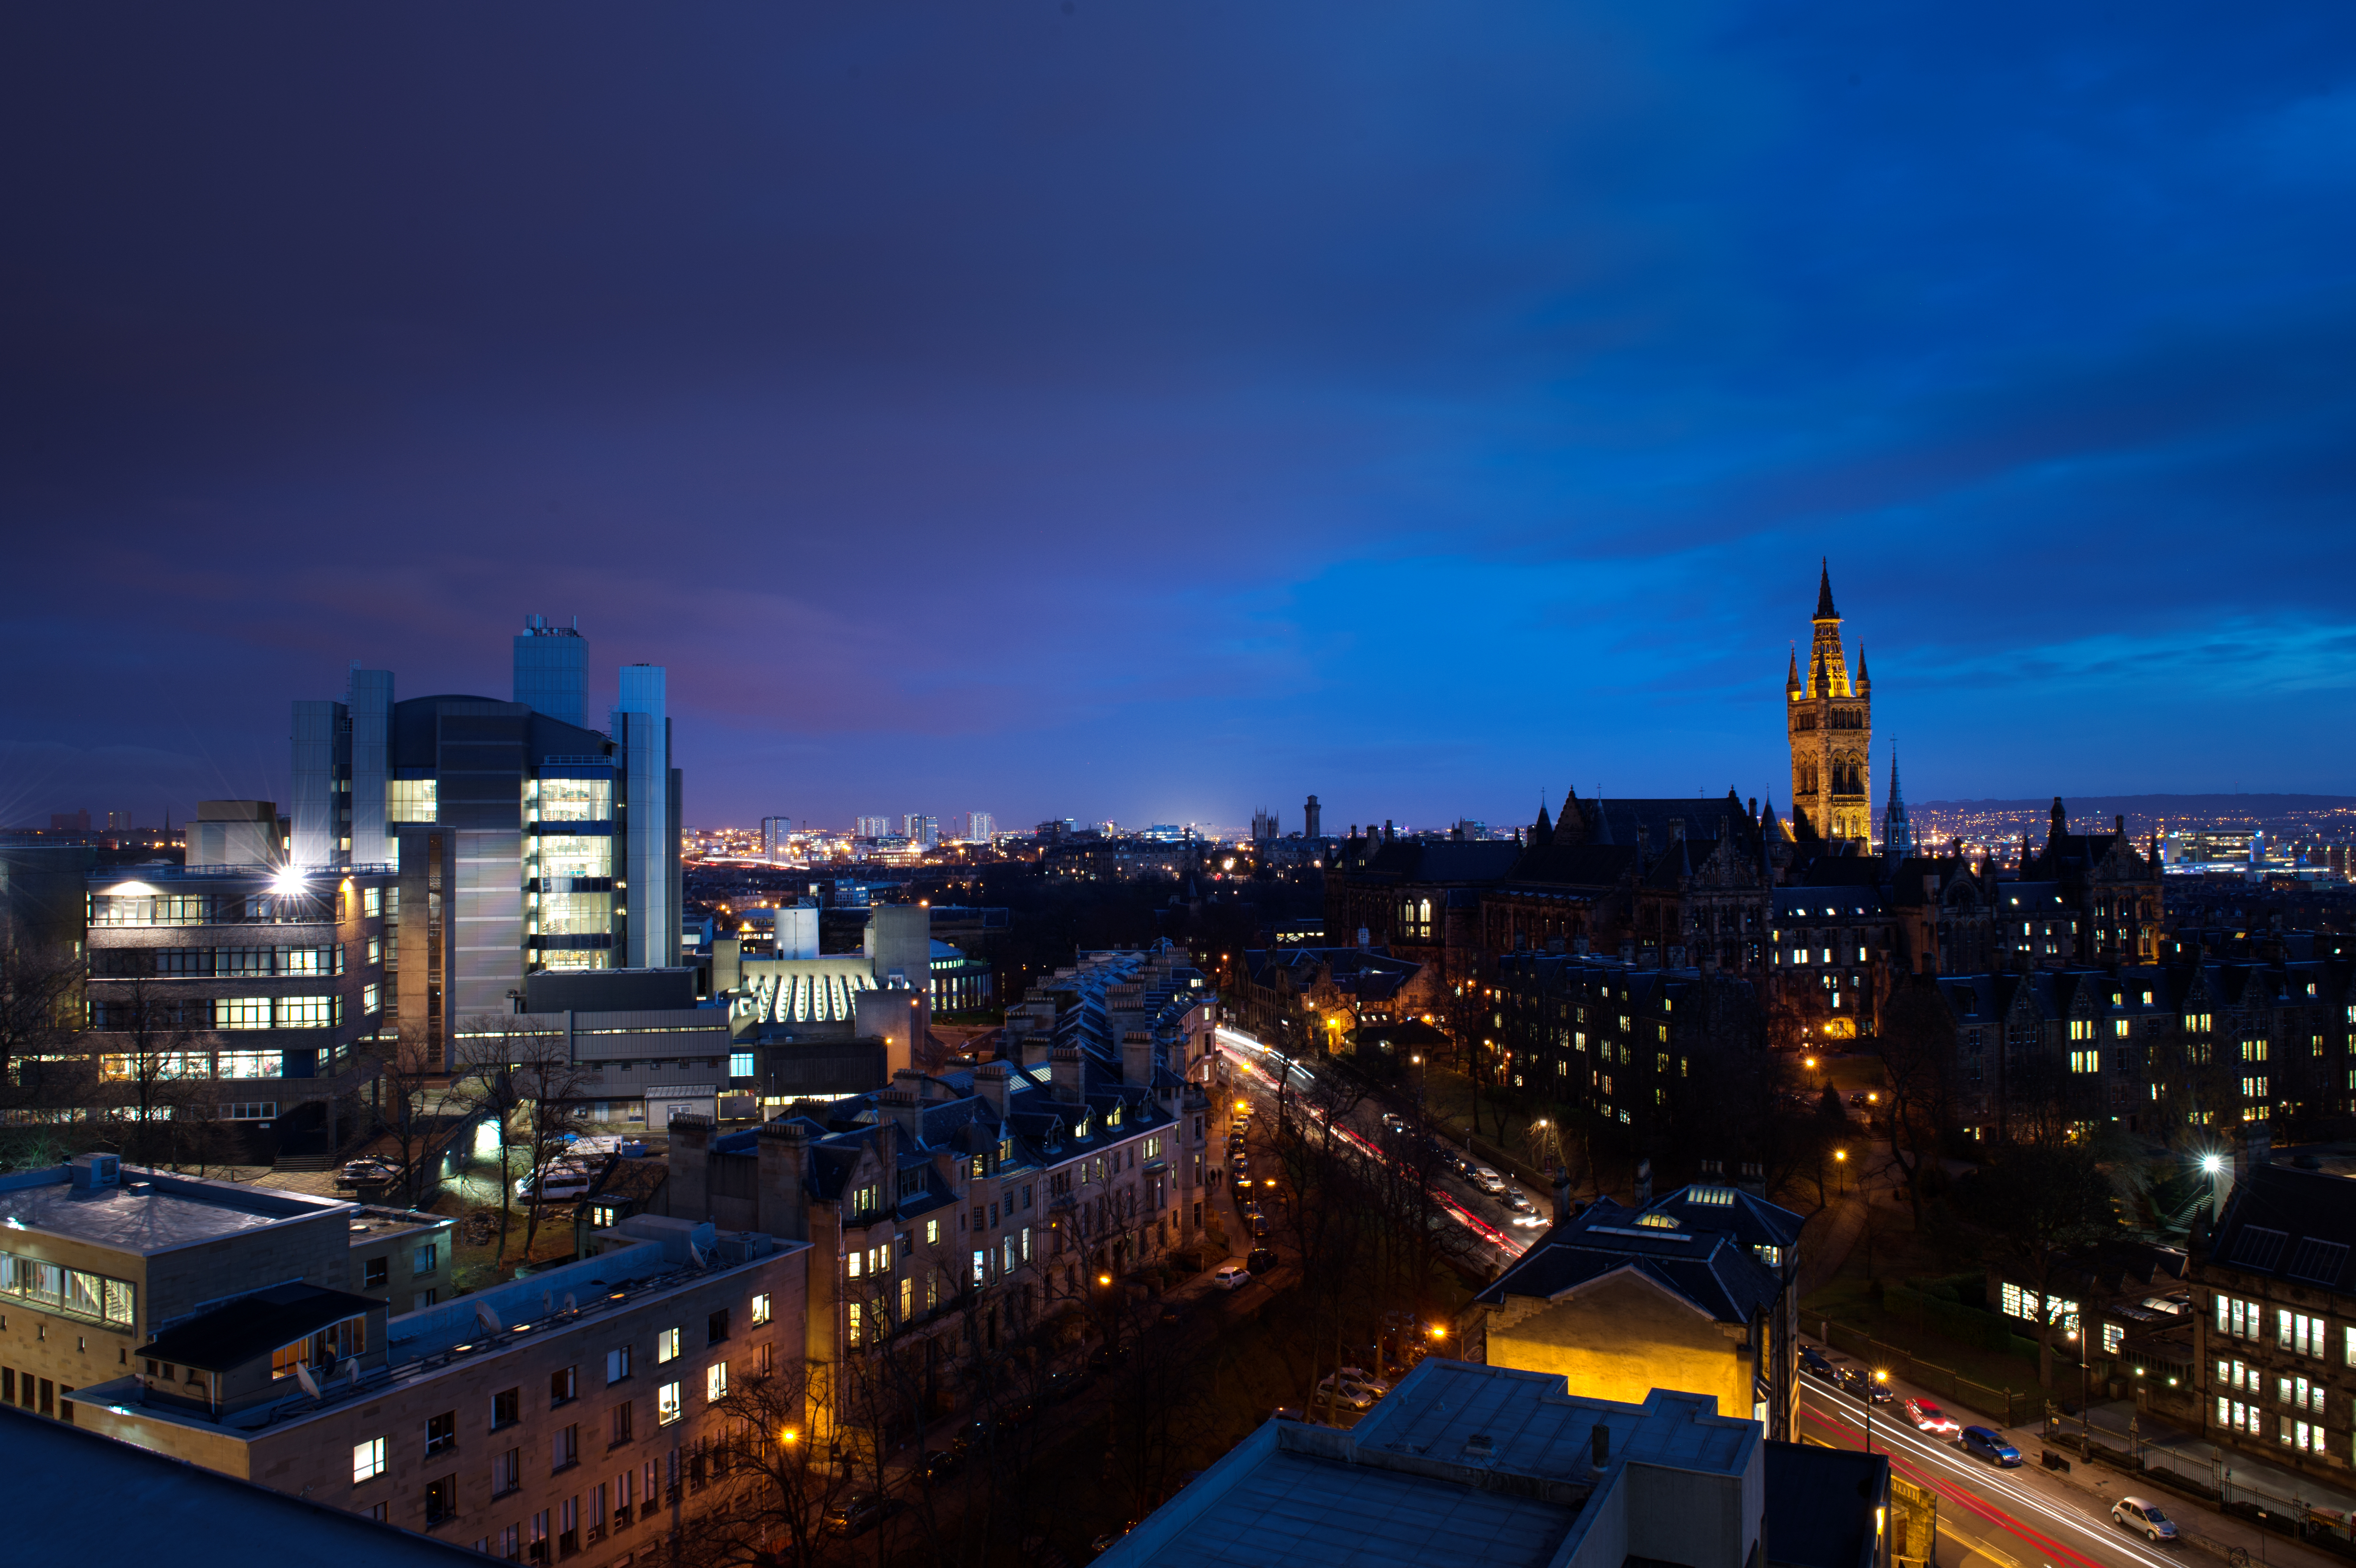
\includegraphics[keepaspectratio=true, width=\paperwidth]{background2.jpg}};
    }

    \begin{frame}[plain,noframenumbering]
        \begin{tikzpicture}[remember picture, overlay]
            \node at (current page.north west) {
                \begin{tikzpicture}[remember picture, overlay]
                    \fill [fill=uofguniversityblue, anchor=north west] (0, 0) rectangle (\paperwidth, -2.6cm);
                \end{tikzpicture}
            };

            \node (logo) [anchor=north east, shift={(-0.6cm,-0.6cm)}] at (current page.north east) {
                \includegraphics[keepaspectratio=true,scale=0.7]{UoG_keyline.pdf}
            };

            \node [anchor=north west, shift={(0.6cm,-0.8cm)}] at (current page.north west) {
                \textcolor{white}{\url{https://ciaranm.github.io/}}
            };

            \node [anchor=north west, shift={(0.6cm,-1.4cm)}] at (current page.north west) {
                    \textcolor{white}{\href{mailto:ciaran.mccreesh@glasgow.ac.uk}{\nolinkurl{ciaran.mccreesh@glasgow.ac.uk}}}
            };
        \end{tikzpicture}
    \end{frame}
}

\end{document}
